\documentclass[border = 0.2cm]{standalone}

%\usetikzlibrary{...}% tikz package already loaded by 'tikz' option
\makeatletter
% Required packages and libraries
\usepackage {tikz}
\usetikzlibrary {patterns}
\usetikzlibrary{calc}
\usetikzlibrary{positioning}
\usetikzlibrary{decorations.pathreplacing}




\begin{document}

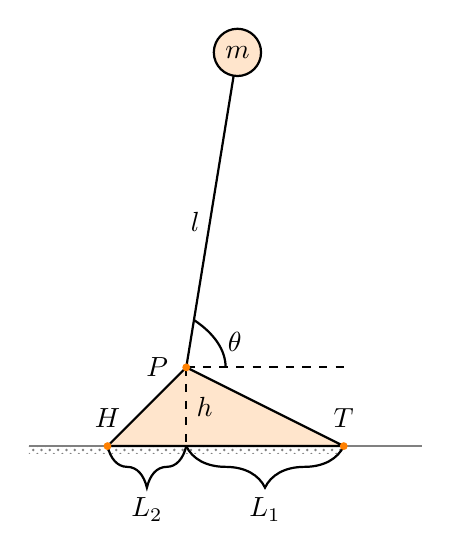
\begin{tikzpicture} [thick]

\newcommand{\point}{0.05};

% ground
\draw [gray] (-2,0) -- (3,0);
\fill [pattern = crosshatch dots,
    pattern color = gray] (-2,0) rectangle (2,-.1);

\coordinate (pin) at (0,1);
\coordinate (pinbase) at (0,0);
\coordinate (mass) at (0.65, 5);
\coordinate (toe) at (2, 0);
\coordinate (heel) at (-1, 0);

% cart
\begin{scope} [draw = black,
    fill = orange!20,
    dot/.style = {orange, radius = .025}]

% \filldraw [rotate around = {-\ang:(0,1.5)}] (.09,1.5) --
%     node [midway, right] {$l$}
%     node [very near end, right] {$m,I$}
%     +(0,2) arc (0:180:.09)
%     coordinate [pos = .5] (T) -- (-.09,1.5);

\filldraw (mass) circle (.3) node {$m$};


% shaft
\draw [-] (pin) -- ($(mass) - (0.048, 0.296)$) node [midway, left] (l) {$l$};

% horizontal dashed line
\draw [dashed] (pin) -- ($(pin) + (2, 0)$);

% theta arc
\draw ($(pin) + (0.5, 0)$) arc
  [
        start angle=0,
        end angle=37,
        x radius=2cm,
        y radius =1cm
    ] node [midway, right] (theta) {$\theta$};


%foot
\filldraw [-] (toe) -- (pin) -- (heel) -- (toe);

%foot height
\draw [dashed] (pin) -- (pinbase) node [midway, right] (h) {$h$};

%foot length
\draw [decorate,decoration={brace,amplitude=15pt,mirror}] (pinbase) -- (toe) node [midway, below, yshift = -15pt] (L1) {$L_{1}$};
\draw [decorate,decoration={brace,amplitude=15pt,mirror}] (heel) -- (pinbase) node [midway, below, yshift = -15pt] (L2) {$L_{2}$};



%pin
\fill [dot] (pin) circle (\point);
\node (P) [left = 0.1 of pin] {$P$} ;

%toe
\fill [dot] (toe) circle (\point);
\node (T) [above = 0.1 of toe] {$T$} ;

%heel
\fill [dot] (heel) circle (\point);
\node (H) [above = 0.1 of heel] {$H$} ;



\end{scope}

\end{tikzpicture}

\end{document}
